
\documentclass[11pt,letterpaper,oneside]{article}
%\usepackage[top=1in,left=1in,right=1in,bottom=1in]{geometry}
\usepackage[top=0.5in,left=1.8in,right=1.8in,bottom=0.7in]{geometry}
\usepackage{textcomp}
\usepackage{fancyvrb}
\usepackage{colortbl}
\usepackage{graphicx}
\usepackage{url}

\usepackage{setspace}
\doublespacing

\title{coDoc: A Tool for Managing Relationships between Code and Documentation}
\author{Dejun Qian\\electronseu@gmail.com}

\date{}

\begin{document}
\maketitle

\begin{abstract}
When writing and testing software, 
lacking of the ability to efficiently refer to the related documentation hinders the productivity largely.
This is particularly true for software that is documentation-intensive, 
such as hardware drivers and virtual device modules.
This paper presents coDoc, 
an integrated development environment for managing relationships between code and documentation, while developing the code. 
We describe the architecture and features of coDoc,
and discuss several design decisions that we faced in developing coDoc and the trade-offs involved in making these decisions.
We report our experiences in mapping two virtual network interface card (NIC) modules to the real NIC documents by coDoc.
\end{abstract}


\section{Introduction}
\label{sec:introduction}
Documents play an important role in the software engineering process,
from requirements analysis to architecture design,
from coding to software testing,
from software debugging to software maintenance.
Software that relates closely to hardware devices is extremely document intensive. % explain why
Examples of such software include bootloaders, 
Operating System (OS) Hardware Abstraction Layers (HAL),
and virtual devices for virtual machines.
Such software must follow the hardware documentation to operate correctly.
A typical embedded CPU might have documentation consisting of thousands of pages.
A computer system usually consists of more than ten hardware modules.
Effectively maintaining the relationships between the code and the documentation is important for developing and verifying such software. % which software

Much work has been done to handle the relationships between Application Programming Interface (API) documents and their client code \cite{Pandita_inferring_2012} \cite{wei_inferring_2011}.
API documents are usually well indexed by the functions or the classes that they define.
When we are interested in a piece of code in the client software,
we can easily find the related API documents by the names of the functions that the piece of code calls.
% The relationships between the client codes and the API documents can be easily constructed by using the function names as the keywords.
However, the code relating to hardware and its documentation usually relate in different ways. % how?
The hardware documents usually talk about how to use the hardware,
more specifically how to program the registers inside the hardware modules.
The hardware documents differ from the API documents in the following ways.
\begin{itemize}
\item the hardware documents are usually published as pdf files, while the API documents are usually html files. % matters?
\item the hardware documents are composed of text, tables and diagrams, while the API documents are usually text only.
\item the hardware docuemnts are not orgnized by functions or classes, which are the basic elements of code, but instead by hardware modules.
\item as a consequence of these differences, it is hard for the computer to relate the hardware document pieces to the code pieces automatically.
\end{itemize}

% These differences make the constructing of the relationships between the hardware related codes and their documents really challenging.
To our knowlege, there are no tools to address this problem.
A simple workaround is to include references to positions of the related documentation as comments in the codes.
However, this can only handle simple situations.
If there are thousands of such comments cluttered in the code,
it will be very hard to manage them.
This paper presents coDoc, a tool to create, maintain, and display the relationships between code and documentation.
% The initial version\footnote{\texttt{\url{git@github.com:derekqian/coDoc.git}}} has been released.
The key features of coDoc are as follows:
\begin{itemize}
\item the ability to display both code and documents;
\item the ability to write and edit code;
\item code pieces selection based on syntax tree of the code;
\item stable code selections regarding to the changes of unrelated codes;
\item creation of relationships between codes and documents;
\item relationships management and display.
\end{itemize}

Using coDoc, we have created relationships between two virtual NIC devices in QEMU and the related documents.
These two devices are DIO \cite{dio} and E100.

The main contributions of this paper are listed as follows,
\begin{itemize}
\item design a framework to display and manage codes, documents and relationships.
\item remain integrity of the relationships when the codes evolve.
\item present a standard format for the code piece identifier.
\item a standard format for the document piece identifier.
\item a standard format for the relationship between the code and document.
\item implement coDoc which adopts these standard formats.
\end{itemize}

The rest of the paper is orgnized as follows. 
Section \ref{sec:background} introduces the background of poppler and CDT.
Section \ref{sec:arch} provides the overall architecture and key features of coDoc.
Section \ref{sec:decision} gives the design decisions of coDoc and the trade-offs of these decisions.
Section \ref{sec:evaluation} summarizes our experiences of creating and maitaining the relationships for two virtual devices.
Section \ref{sec:related} presents the related work.
Section \ref{sec:conclusion} concludes our work and gives some thinking towards the future.


\section{Background}
\label{sec:background}
\subsection{poppler}
We adopt poppler, a open-source PDF render, to render PDF content in coDoc.
This PDF render is written in C++, 
and is widely used in Linux systems.
It uses Cairo and GTK to draw the rendered content.

\subsection{C/C++ Development Tool}
C/C++ Development Tool (CDT) is an Eclipse plugin which supports C/C++ syntax parsing.
It is written in Java and provides Eclipse with the ability of syntax highlighting and code completing when developing C/C++ codes.



\section{Architecture and Features of coDoc}
\label{sec:arch}

\begin{figure}
\begin{center}
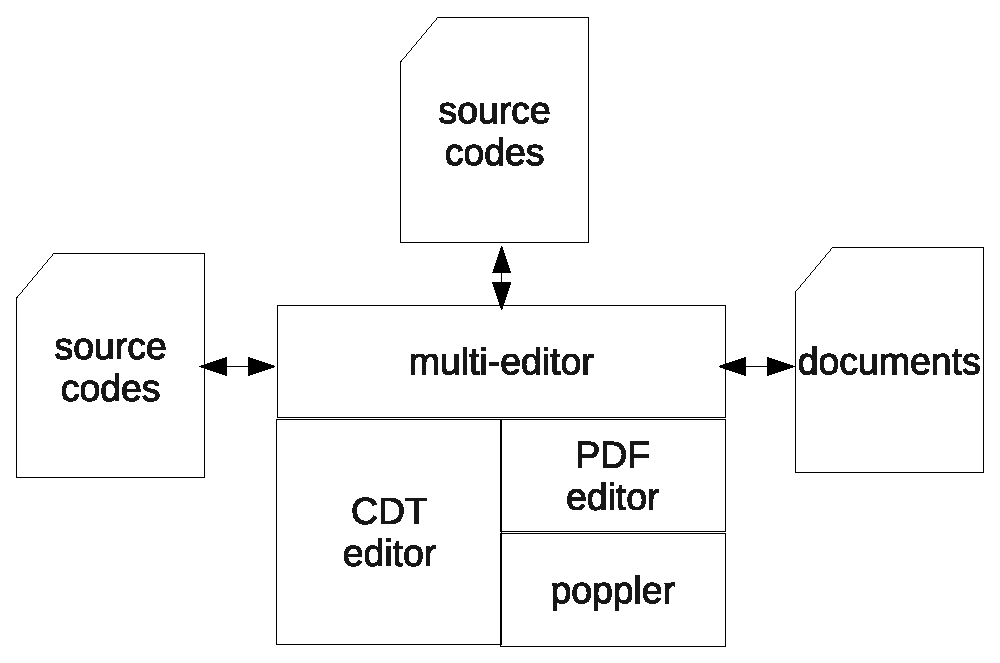
\includegraphics[width=0.55\textwidth]{architecture.eps}
\caption{coDoc Architecture and Features}
\label{fig:architecture}
\end{center}
\end{figure}

The architecture of coDoc is shown in Figure \ref{fig:architecture}. 
It contains CDT editor, poppler, PDF editor and multi-editor.
There are three kinds of data here, 1) the codes, 2) the documents, 3) the relationships.
We only handle C/C++ code at this time, 
as most system code are written in this language.
CDT editor reads and parses the codes, 
highlights syntax elements.
We use poppler to read the PDF file and render the PDF pages to images.
As poppler is developed in C++, and Eclipse RCP is in Java language,
we need an adaptor to bridge the C++ code and the Java code.
We use JNI to implement this adaptor.
PDF editor implements an adaptor, 
and uses it to get the PDF page from poppler and displays the page.
The multi-editor is responsible to read the relationship data,
and highlight certain code piece and document piece respectively.
To represent a relationship, 
we first need to define the strategy to identify the code piece and document piece.


\subsection{Identifying the Code Piece}
The codes are always evolving during its lifetime.
We don't want our relationships created for one version stop working for other versions.
This goal calls for a robust identifying strategy for the code piece.
Our first method identifies the code piece as the offset of the selected code from the beginning of the code file and the selected length.
This method is straight forward and is easy to understand and implement.
However, this method definitely will violate the robust requirement.
To achieve the goal, we need to find some properties of the code that are relatively stable when code evolves.
These properties should also can serve as a key to uniquely identify the code piece.
The intuitive thought is to use the semantic information,
as it describes the intrinsical meaning of the code.
However, there is no formal method to describe this information.
We use syntax information to form the main element of our identifier.
The code can be parsed and represented by a syntax tree.
The change of the code in one branch will usually not affect the code in the other branches.
If we can identify the code piece based on the position in the syntax tree,
we can design a robust method to identify the code piece.
To make the method more robust,
we can introduce the information in the first method as the secondary key.
When the syntax identifier fails to locate the code piece,
we can use the offset information to assist the decision.
We also include in the identifier the content of the code piece for the integrity check.
The structure used to achieve this goal is shown bellow,
\begin{Verbatim}[frame=single]
class CodeSelection {
  private String syntaxcodepath;
  private String selcodepath;
  private String syntaxcodetext;
  private String selcodetext;
}
\end{Verbatim}


\section{Methodology and Design Decisions}
\label{sec:decision}
\subsection{Embedded vs Seperate for PDF Reader}
The tool should display both codes and documents at the same time.
We can implement the code viewer and the PDF viewer in seperate process,
and use inner process communication (IPC) techniques to synchronize.
The advantage of this method is that each process has its own window,
can ocuppy the whole screen,
and display more content which reduces the need to scroll the window horizontally.
When the user uses a computer with two monitors,
the tool implementing this method is extremely a good choice,
as the user can choose to display the code and the document in seperate moniter.
However, this implementation is heavy,
and get performance issues.
When using the tool, 
the user may need to launch the PDF reader,
which is slow.
Our earlier implementation use this method,
and encountered a lot of synchronization problems oriatated from the IPC communication.
In coDoc, we choose to implement the code viewer and the code viewer in the same process.
This way, all the commucations are done in the same process.
%The Eclipse framework even makes the whole system single thread.
No IPC communication is needed,
which is more efficient and makes the tool more user-friendly.
With the new method, we can smoothly operate the tool without any uncomfortable feeling.
The advantage of the first method become the disadvantage of the new method,
as the code viwer and the document viwer should share the whole screen now.
However, with a efficient and user-friendly screen split strategy and screen area assignment method,
we can make the user feel less uncomfortable when viewing the content.
Also, most programmer now not only are using two moniters, 
but also the moniters they are using are larger and larger.
Using a larger moniter with high definition will make this disadvantage nothing.
And even better, in this situation, this method will overcome the first method,
as moving the eyes between two big moniter is energy consuming.

\subsection{Relationship Store Model}
In coDoc, we store the relationship data in XML file, 
instead of the SQL database.
The reason that we didn't use a SQL database is that the relationships is semi-structured,
as we decide to store the content along with the identifier.
The content is used to further check the integrity.
XML database is very suitable for our semi-structured data here.


\section{Evaluation}
\label{sec:evaluation}
\textbf{Effectiveness.} We have evaluated coDoc by mapping two virtual devices and their related documents.
The number of relationships created and the time used to created these relationships are listed in Table \ref{table:evaluate}.

\begin{table}[th]
\caption{Evaluate Result}
\centering
\begin{tabular}{rcc}
\hline
Code & \# of Relationships & time(hr) \\
\hline
dio & 108 & 2 \\
e100  & 213 & 4\\
\hline
\end{tabular}
\label{table:evaluate}
\end{table}

The fine granularity of the identifying method makes the relationship results very accurate, 
80\% of the code pieces are marked inside the statement.
This result is hard for comment-based method to achieve.
The same result happens for the document.
In the whole relationships, 
90\% of the document pieces are marked on cells in the tables.
The comments in the PDF file will be too crowd to be useful,
as it will affect the normal reading of the document.
Our approach can also make the development efficient,
as we don't need the developer to change either the code or the document while only relationship is created.
This makes the code and document neat and easily to read and understand.

\noindent \textbf{Usability.} We implement coDoc as an Elipse\footnote{\texttt{\url{http://www.eclipse.org}}} Rich Client Program (RCP), 
which can make our tool share the use style with Elipse that is acustomed by many programmer.
Figure \ref{fig:platformview} is the screenshot of the tool.
Three persons with no exprience with coDoc before have successfully use this tool to create the relationships for their codes and documents.
They didn't find any difficulties when using this tool.
All the feedbacks are positive regarding to the use of the tool.
Now they can easily create their relationships by selecting the code and document piece using mouse, input the comment using keyboard.
They can also manage the relationships by sorting by attributes, search certain relationships by keywords.
They also find the feature that allow them to categorize the relationships helpful.
This feature makes the relationships more neat when the number of relationships is large.

In our own experience, we found that the ability to see the codes, 
the documents and the relationships in the same screen really saves a lot of time,
as we don't need to switch between different tools.
The visualized interface also saved us time to learn the detailed syntax about the identifier formats,
and to write the identifier manually.
We believe this tool will lead to increased productivity.

% convert platformview.png platformview.eps
\begin{figure}
\begin{center}
\includegraphics[width=\textwidth]{platformview.eps}
\caption{coDoc Platform View}
\label{fig:platformview}
\end{center}
\end{figure}


\section{Related Work}
\label{sec:related}
Current tools can manage codes. 
These kinds of tools include revision control software like git, svn. 
Revision control tools can give the evolving history of the software.
These tools usually adopt text comparison tools to figure out the differences between different versions of the software.
The comparation tools can easily give the result about the matching points and mismatching points in the codes,
which means they can manage the relationships between different versions of codes.
However, these tools are not designed to manage documents.
Though some people also use them to manage documents,
they only use it as a persistent data warehouse.
They can not take the advantages of the comparison tools, 
as these tool usually can only deal with text file.
People are using code comments to record the related document piece.
However, no consistent format exists,
which makes these information not managable,
especially when these comments are made by many different developers.

Full text indexing system is developed to processing documents.
However, they can only relate keywords to certain documents.
They do not deal with both codes and documents. 
Like full text indexing system,
search engines also work with documents in similar way.
Most of the documents that are handled by search engines are web pages.
Many PDF readers can support highlighting and commenting.
With these features, we can relate a document piece to a code piece.
However, these links created are not stable,
and PDF readers can not check the integrity of these information.

Generally speaking, these are tools can either do code management or do document management.
However, they are not designed to do both,
and managing the relationships between codes and documents is definitely a mission impossible task for them.


% Based on what you have so far, what can you conclude?  What cool ideas did you think up but not have time to implement so far?
\section{Conclusions and Future Work}
\label{sec:conclusion}
We implement coDoc, 
a tool to managing the relationships between the hardware related codes and their documents.
The main contributions in this paper are the method to identify the code piece.
Our experiences of using coDoc to manage two virtual device codes and their documents show the tool is robust and efficent,
and is helpful when developing and maitaining the virtual devices.
The relationships remain stable respect to the evolution of the codes.

There are still opportunities to improve coDoc, 
\begin{enumerate}
\item combine it with revision control tools to provide a more user-friendly tool suit for developing and maitaining the codes while managing the documents at the same time.
\item more robust method to identify the document pieces in the PDF documents to make the tool invariant to the change of the documents.
\item use machine learning method (use the data created as seed to train the model) to construct and check the relationships between hardware related codes and their documents.
\end{enumerate}



% Follow a standard ACM format for your references.  You have examples in the papers you have read.
\bibliographystyle{acm}
\bibliography{reference}

%\begin{thebibliography}{9}
%\bibitem{bib:coDoc}
%\emph{http://www.coDoc.org}
%\end{thebibliography}

\end{document}
